\documentclass{paper}
\usepackage[onehalfspacing]{setspace}
\usepackage[a4paper, total={6.25in, 9in}]{geometry}
\usepackage{amsmath}
\usepackage[numbers]{natbib}
\usepackage{graphicx} 
\graphicspath{ {images/} } 
\usepackage{float}
\usepackage{listings}
\usepackage{color}

\title{Emergence and Collapse in Dissipative Dynamical Systems \\ \textnormal{Spring 2019 Network Science Project}}
\author{S. Migirditch, TF. Varley}

\begin{document}
	\maketitle
	
	\section{Introduction}
	The second law of thermodynamics captures how local decreases in entropy can facilitate global increases. This provides a mechanism for the spontaneous emergence of structure in systems. Far from equilibrium dynamics are mathematically difficult to study, partially because the second law gives no deterministic insight into the dynamics of transient emergent behavior beyond motivating its existence. The few other theoretical tools available like Crooks theorem \cite{crooks_entropy_1999} place only weak restrictions on possible transient behavior.
	However the complex systems found in nature ranging from whirlpools to evolved life manage to develop increasing complexity with relative stability. In the absence of theoretical fire power, some conceptual framework can give limited experimental guidance. Diffusion driven emergence is caused by the dissipation and equilibriation of a resource. If there is no resistance to diffusion no structure will emerge. Therefore it is the structure and dynamics of the system which the resource is diffusing through that exclusively determines the properties of emergent phenomena\cite{strogatz_exploring_2001, gates_control_2016}. This concept has been used with varying degrees of acknowledgment in several experimental designs. Of particular interest to this project is the computational network ecology work based on the niche model \cite{Williams2000}. The primary purpose of this work is to explore the properties inherent to the niche model rather than the parameters of the broader systems it is incorporated into. A secondary focus is discovering the set of dynamics that can be produced by a very general model of competitive resource consumption in a network structured by the niche model. 
	\section{The Model}
	
	The model and all analyses where programmed in Python 3.6, using the NetworkX package, version 2.2, as provided by Anaconda. The complete code needed for reproduction is included in Appendix 1.
	
	
	\section{Analyses}
	
	We ran a series of analyses on the developing network at every moment in time. The most basic where analyses of the degree distribution: the total number of nodes at each moment, the mean, variance, and standard deviations of the degree distribution at every moment, and the normalized Shannon entropy, which was calculated as:
	
	\[ H(G) = \frac{1}{N}[-\sum_{0}^{i} p_{i}log_{2}(p_{i})] \] 
	
	where $p_{i}$ is the probability of each degree and $N$ is the number of nodes in the network. We also calculated graph properties of the network at each timestep, including the average clustering coefficient, the global and average local efficiencies, the algebraic connectivity (defined as the eigenvalue of the second eigenvector the graph Laplacian), and the average harmonic centrality.
	
	Finally, for each node, over the course of it's life, we tracked the average volume it consumed, the average local efficiency, the average harmonic centrality, and the average in- and out-degrees. This allowed us to estimate what sorts of relationships between nodes most allowed individuals to live the longest. 
	
	The simulation ran until either one of two conditions was met: there were fewer than 3 nodes left in the network, or the system had run for 100 timesteps. Typically, the network had collapsed down to $<$3 nodes by about 50 timesteps. 
	
	\section{Results}
	
	
	\subsection{Whole-Network Measures}
	The most basic network measure we tested was the population over time. For a visualization, see Figure \ref{population} We found that the network displayed a very stereotyped evolution through time. There was typically a period of initial growth, which ended with a small die-off, or extinction event, which decreased the population. Following that, the population showed a smooth, exponential growth until the resource node was exhausted. After the resource node was exhausted, the network quickly began to collapse, showing an increasingly steep population collapse. 
		
		\begin{figure}[h]
			\centering
			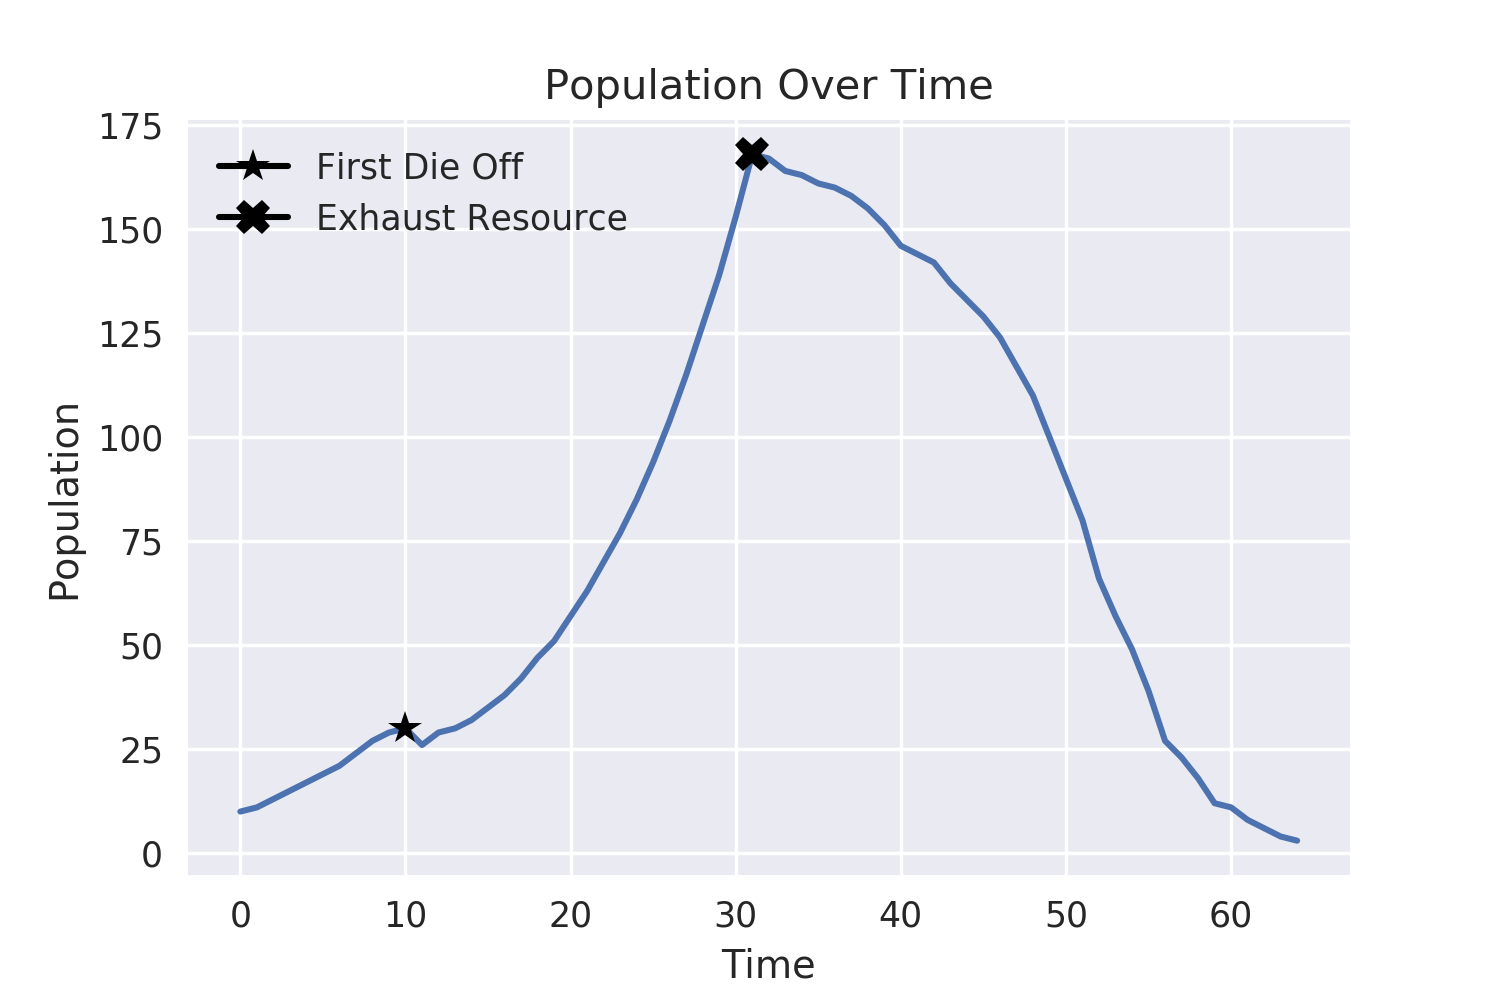
\includegraphics[scale=0.75]{population.png}[H]
			\caption{The number of nodes in the network through time. Notice that there are two local maxima: an early die-off, indicated with a $\star$, and the global maxima, indicated with an \textbf{\textsf{x}}}.
			\label{population}
		\end{figure}
	
	To characterize the degree distribution, we calculated the mean and standard deviation of the degree distribution over time, as well as the variance, and the normalized Shannon's entropy. The mean and standard deviations, and the variance (Figure \ref{mean-std}) showed similar changes over time to the population: a spike in mean degree and standard deviation near the early die-off, followed by a much shallower recovery that peaked when the network exhausted it's resource node. The variance showed a similar pattern, with a dramatic peak right before the die-off. Both the mean degree and the variance of the distribution began to become erratic as the network decayed. 
	
		\begin{figure}[h]
			\centering
			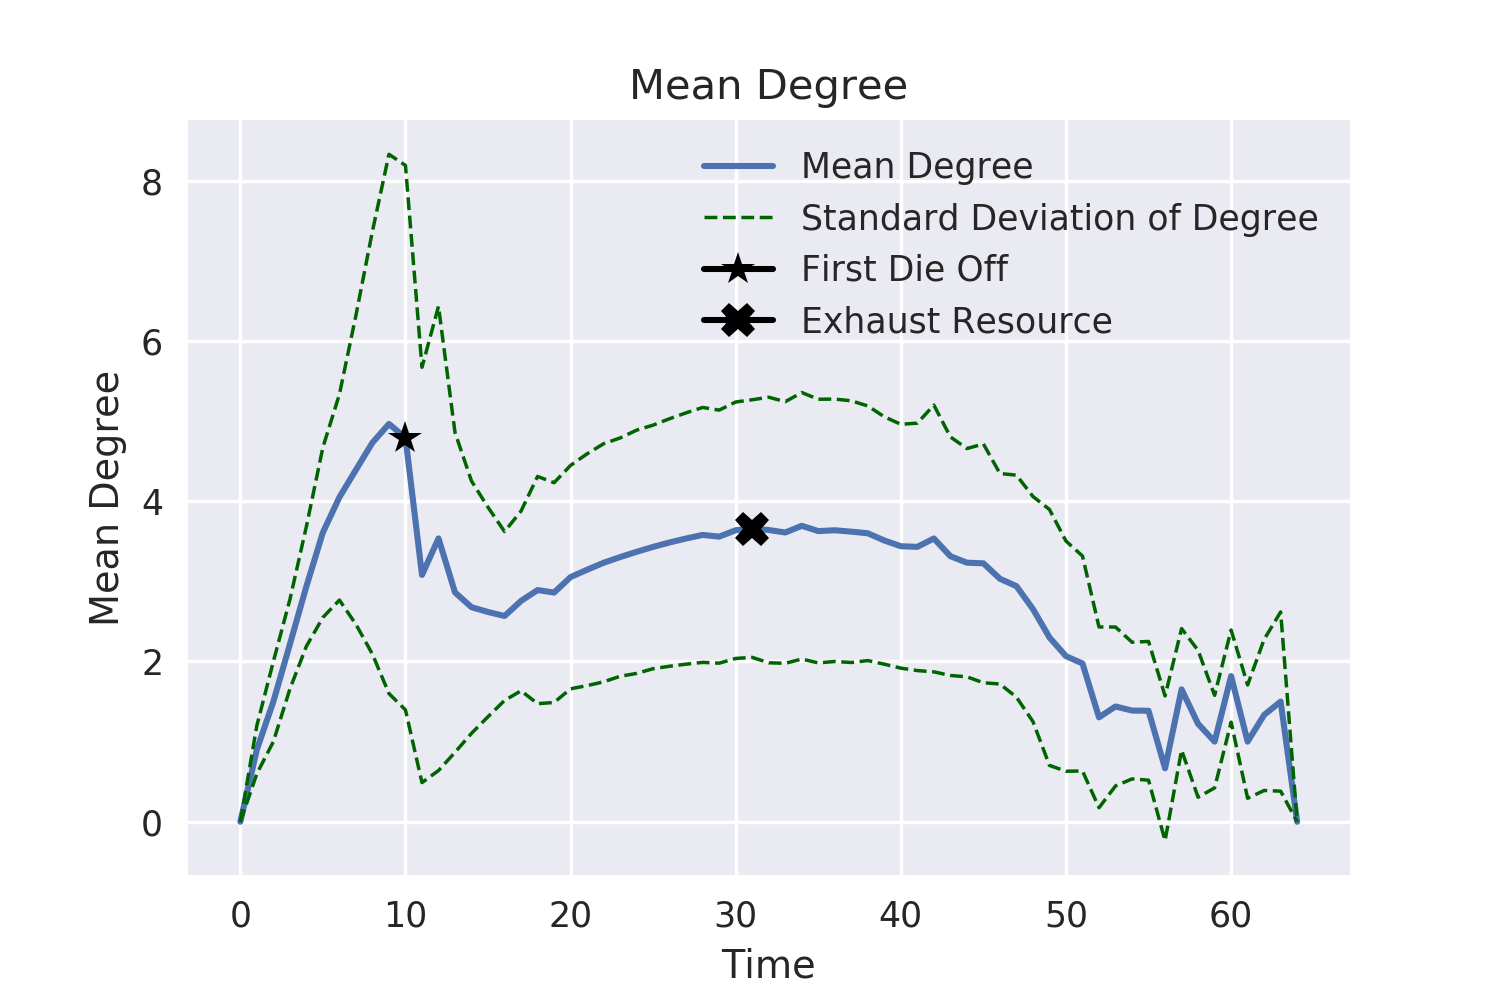
\includegraphics[scale=0.75]{mean_std_degree.png}
			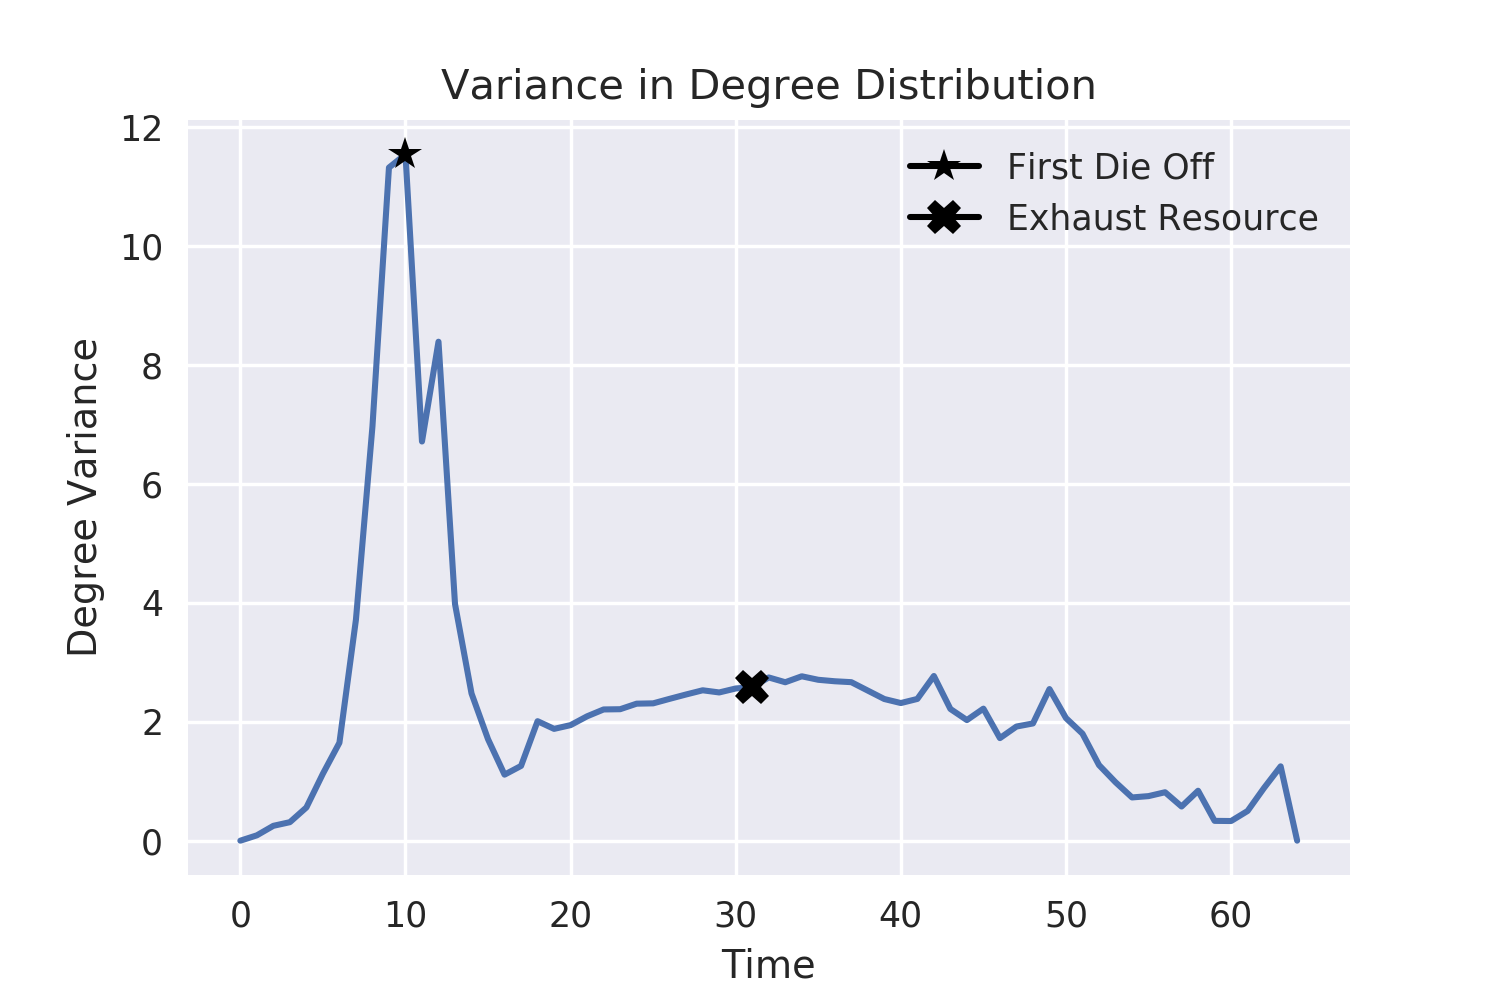
\includegraphics[scale=0.75]{variance_degree.png}
			\caption{The mean degree of the network at each timestep $\pm$ one standard deviation and the variance of the distrubiton at each moment. As with the population, two distinct local maxima are visible: both the mean degree and the variance in the degree distribution peak immediately before the early die-off and then collapse, before recovering to a smaller, broader peak at the moment of resource exhaustion.}
			\label{mean-std}
		\end{figure}
		
	The normalized Shannon entropy of the degree distribution showed a very similar pattern (see Figure \ref{entropy}), although with intriguing differences. Instead of climbing, as variance and mean degree do as the network develops, entropy falls, reaching a local maxima near the die-off, and a nadir when the resource node is exhausted. This is somewhat unexpected: we might interpret this to indicate that, near the peak of network development, the structure has a very 'lattice-like' topology, which most nodes connecting to similar numbers of other nodes. It is also possible that, as the normalization term increases with network size, that comes to dominate, dragging down the overall value. This finding strongly suggests that the dissipative process is not simply building a 'random' network through time: the dynamics of the process seems to constrain the structure of the network to a more globally ordered state. This is an excellent validation of the dissipative structure concept and implementationn. 
	
	\begin{figure}[h]
		\centering
		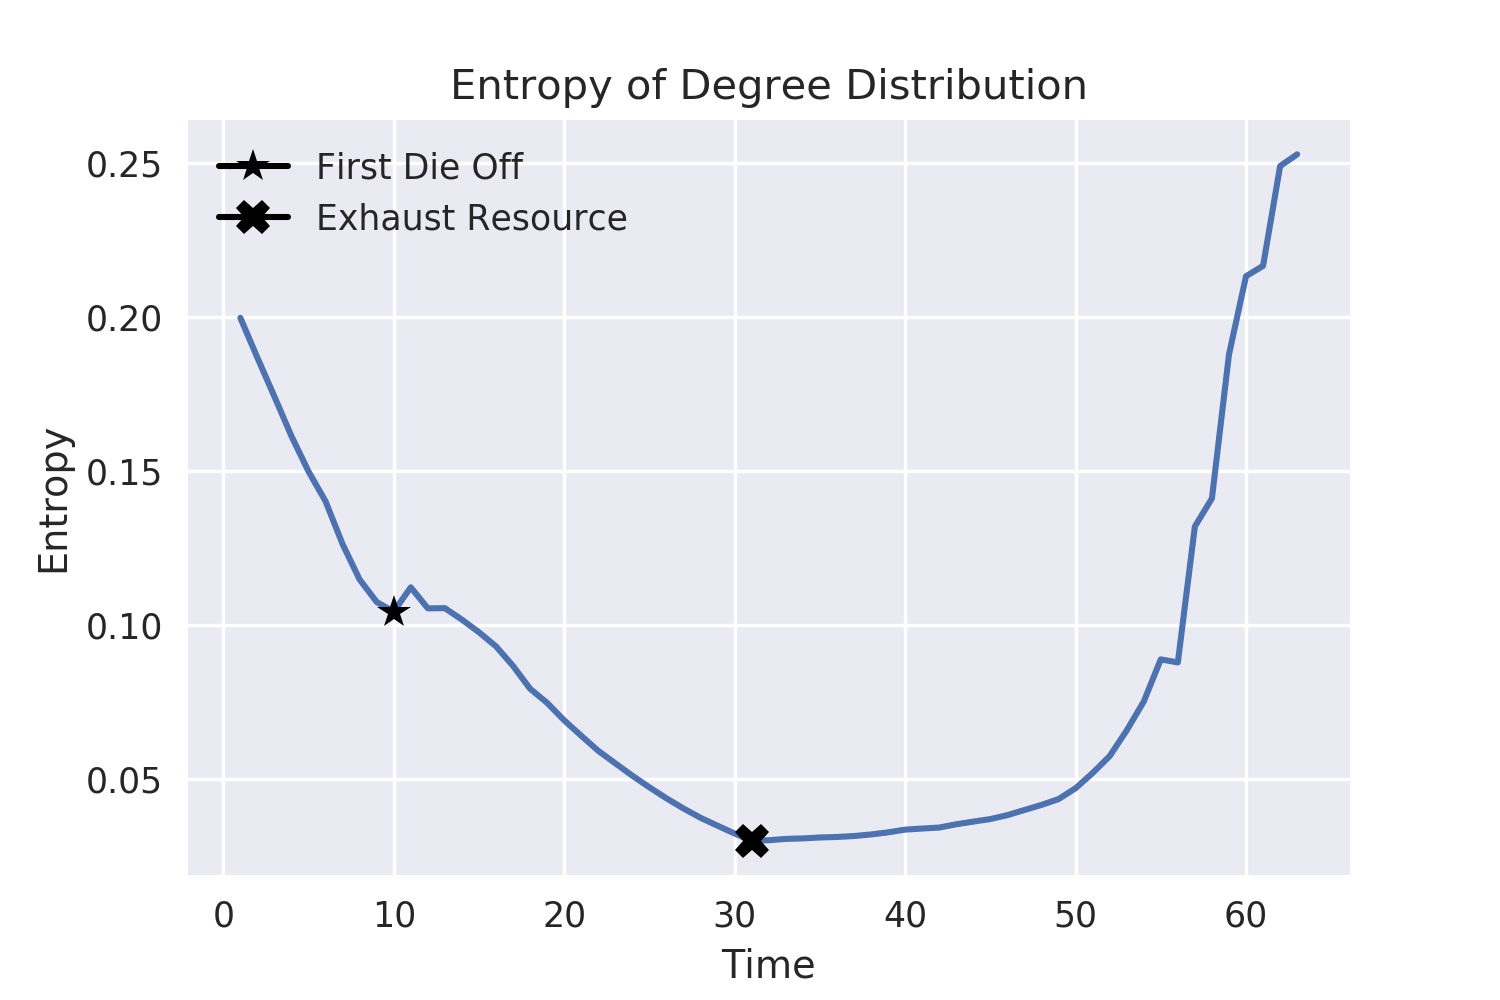
\includegraphics[scale=0.75]{entropy_degree.png}
		\caption{The normalized Shannon entropy of the degree distribution over time. In contrast to other measures like variance or mean degree, normalized entropy falls as the network develops. }
		\label{entropy}
	\end{figure}
	
	Over the course of the lifetime of the network, particularly after the resource node was exhausted, we were interested in how the network decayed. We had two competing hypothesis about how the network could collapse: Hypothesis 1 was that the network would fragment along weak ties leading to multiple, high-connected modules that would in turn fragment into nothing. Hypothesis 2 was that the network would collapse from the fringes in, maintaining a single connected component, which would loose periphery nodes over time. In Figure \ref{components}, we can see that, for most of the networks lifetime, the network is dominated by a single, giant component, which persists for quite a bit of time after the network has exhausted the resource node. There seems to be a critical point, however, where the network rapidly collapses into many disconnected components, that quickly decay into small chains of individual nodes or pairs. This suggests a mixture of both Hypothesis 1 and Hypothesis 2: for as long as the network is able to maintain a certain level of flux through it, a giant component can be maintained, however, once that level is lost, the network very quickly fragments. 
	
	\begin{figure}[h]
		\centering
		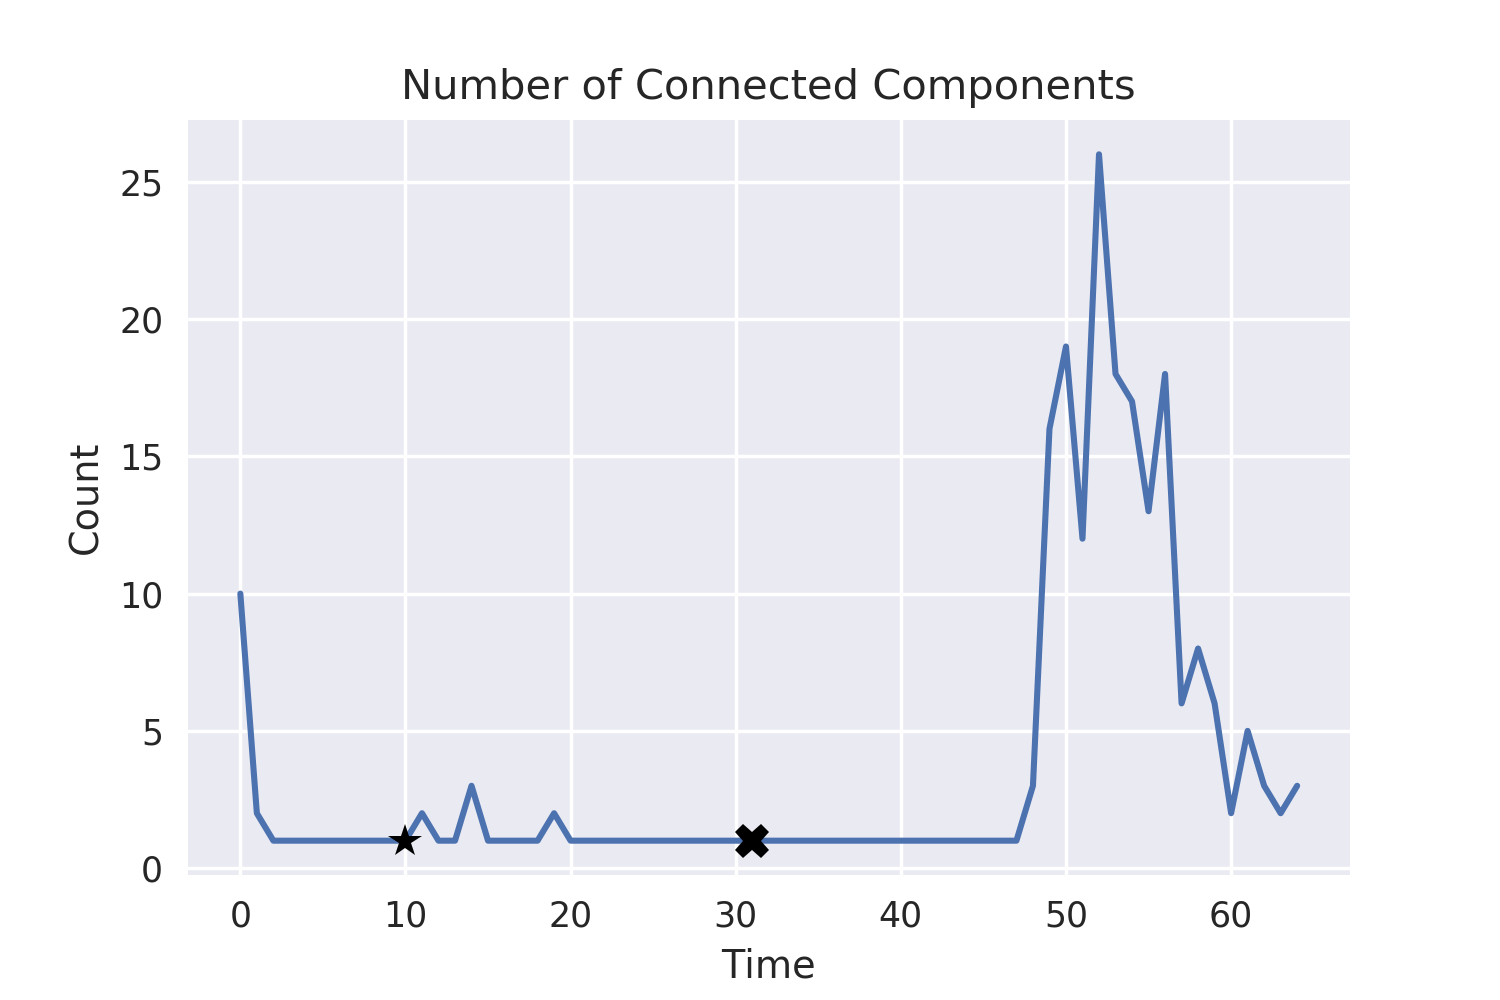
\includegraphics[scale=0.75]{num_components.png}
		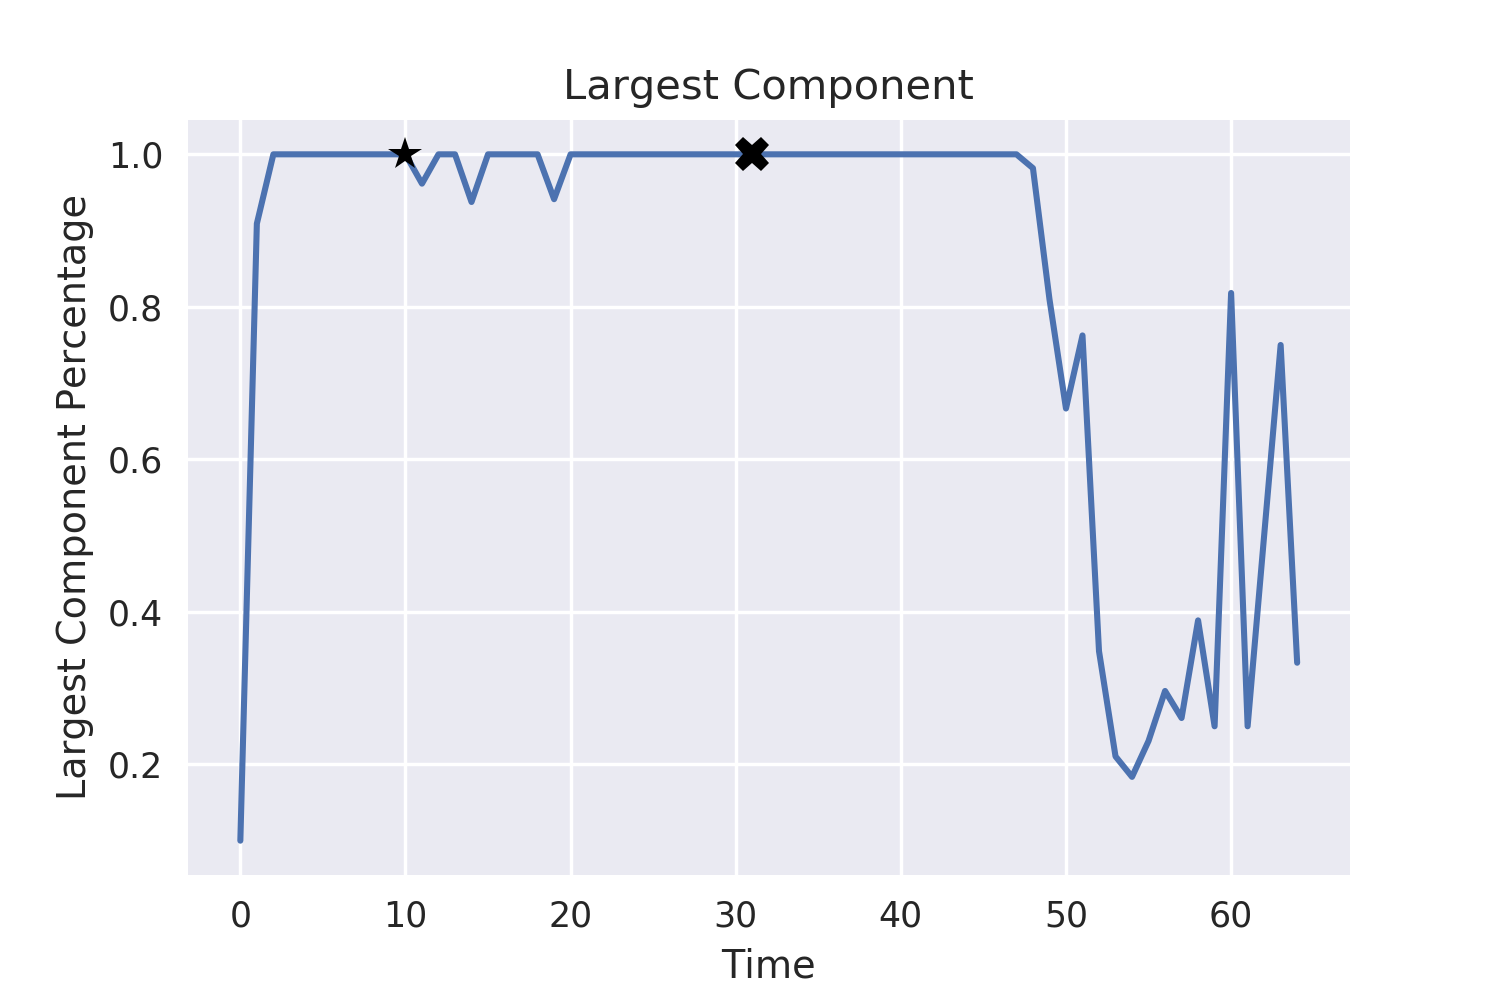
\includegraphics[scale=0.75]{largest_component.png}
		\caption{The number of connected components in the network over time, and the fraction of the total number of nodes contained in the largest component over time. In the upper plot, we can see that the network maintains a single, core component throughout most of it's life (the small bumps between time 10 and 20 are new nodes that have been added, but not yet connected to the main core). The network remains a single, connected component until what seems to be a critical point near time 50, at which point it quickly fragments into many smaller components, few of which dominate the set the available nodes.}
		\label{components}
	\end{figure}
	
	As the network evolved and fragmented, we calculated the edge density, which was defined as the number of existing edges, divided by the number of possible edges. Interestingly, we found that the edge density was highest before the initial die-off, and towards the very end of the systems life (see Figure \ref{density}). At no point does the network become particularly dense, like most real-world networks, it remains spares throughout. The finding that it was maximally sparse near the peak of network development is interesting, but not entirely unexpected, since nodes do not necessarily connect to more neighbours than is necessary to keep them alive. In the context of a natural system, this could be considered a form of specialization: most animals don't evolve to be able to consume more different species than they need to to survive. Similarly, in economic systems, firms will buy the smallest amount of product necessary to turn a profit on whatever they are producing. Sparsity is efficient. 
	
	\begin{figure}[h]
		\centering
		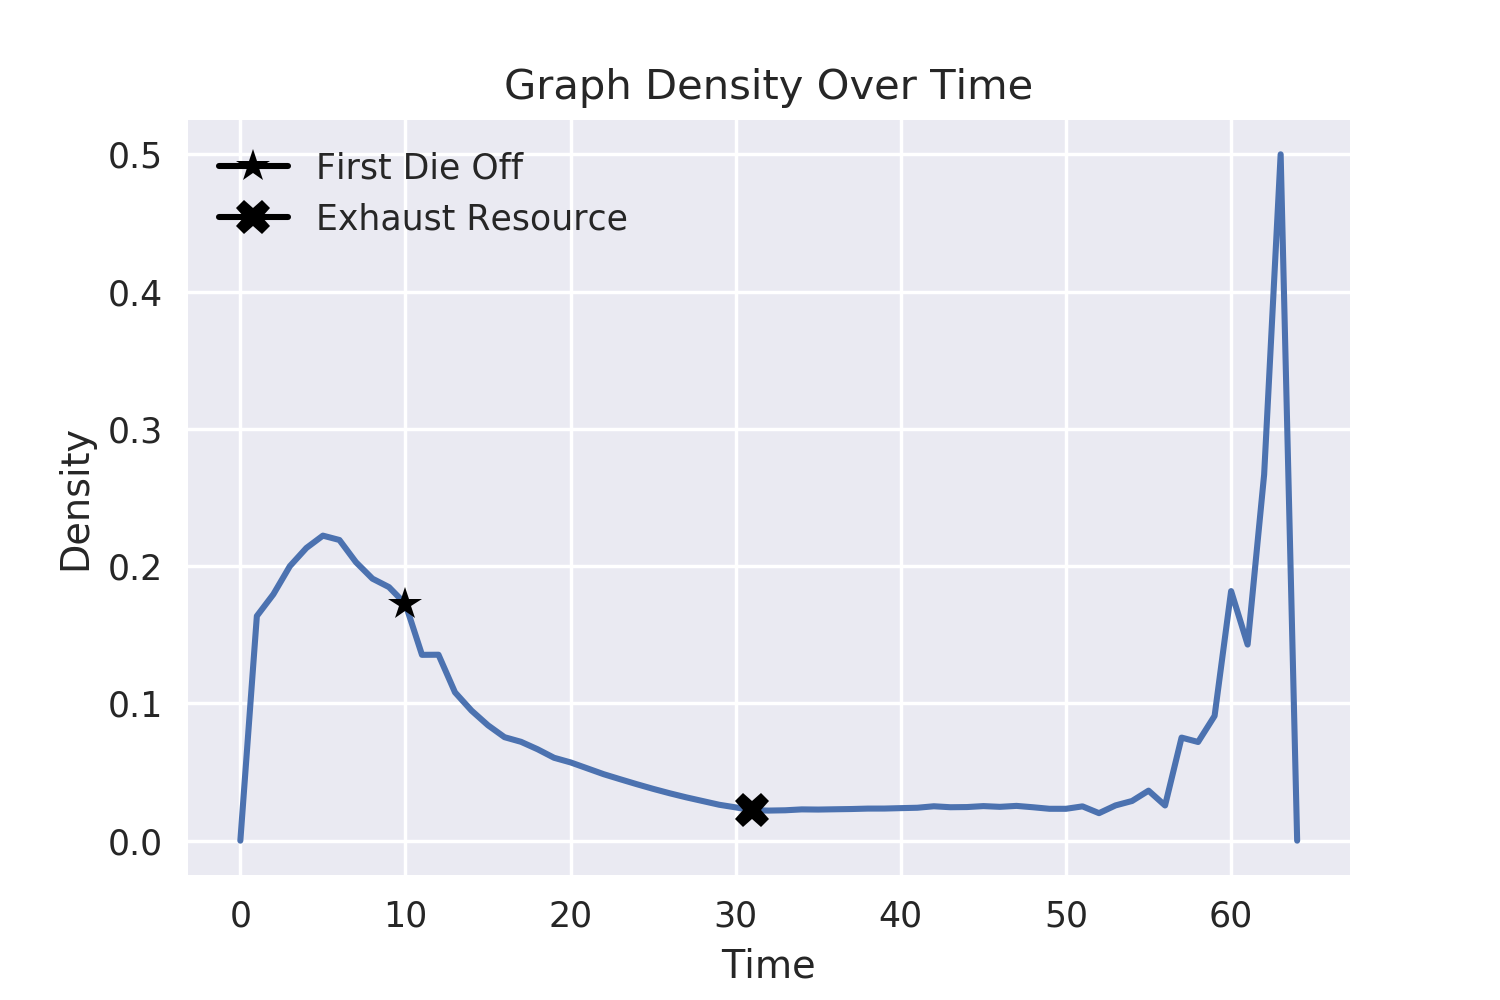
\includegraphics[scale=0.75]{density.png}
		\caption{The density of the graph, defined as the number of existing edges, normalized by the total number of possible edges. The spike in density before the initial die-off was unexpected, although the later spike is more easily explained, as the number of nodes in the network shrinks to nothing, so the number of possible edges does as well.}
		\label{density}
	\end{figure}
	
	We also looked at algebraic connectivity, local efficiency, global efficiency, and average harmonic centrality. 
	
	\begin{figure}[h]
		\centering
		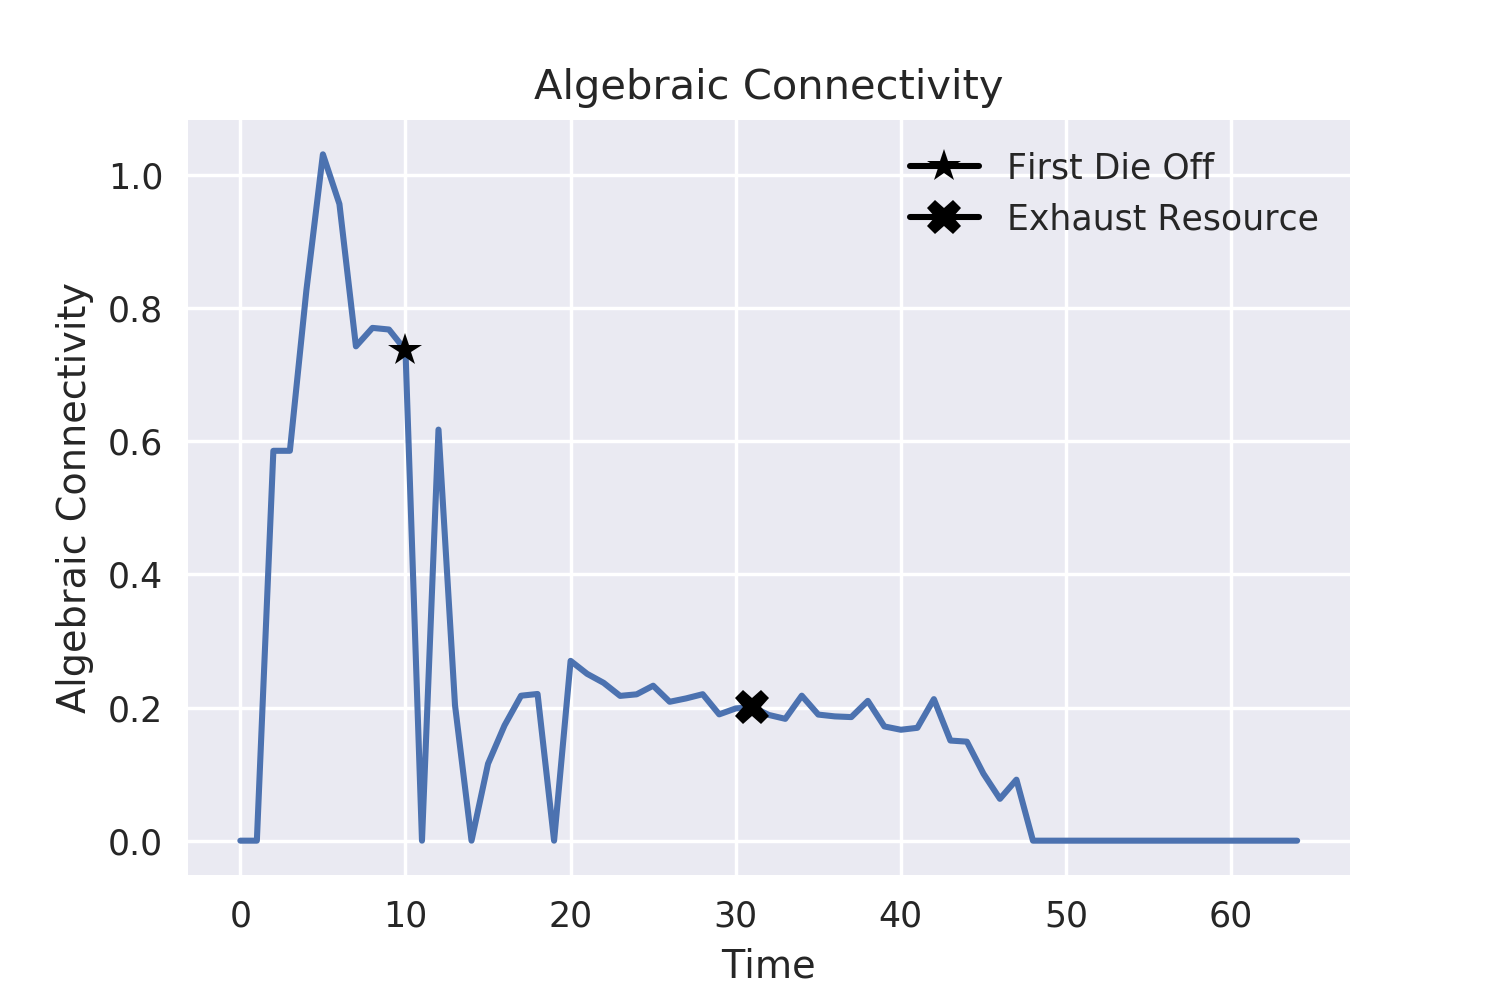
\includegraphics[scale=0.75]{alg_conn.png}
		\caption{The algebraic connectivity of the graph over time. Algebraic connectivity is greater than 0 only when the graph is fully connected, so any moment where the graph is not, the plot drops to zero. The moments between time 10 and 20 where the plot drops match the brief moments of disconnection that can be seen in Figure \ref{components}. Despite these brief drops, an overall pattern is clearly visible: algebraic connectivity spikes just prior to the initial die-off, and then falls, slowing as the graph reaches it's maximal size. Most interestingly, algebraic connectivity begins to drop more precipitously right before the graph becomes fully disconnected, suggesting that it may predict total collapse slightly before it begins.}
		\label{alg-conn}
	\end{figure}
	
	\begin{figure}[h]
		\centering
		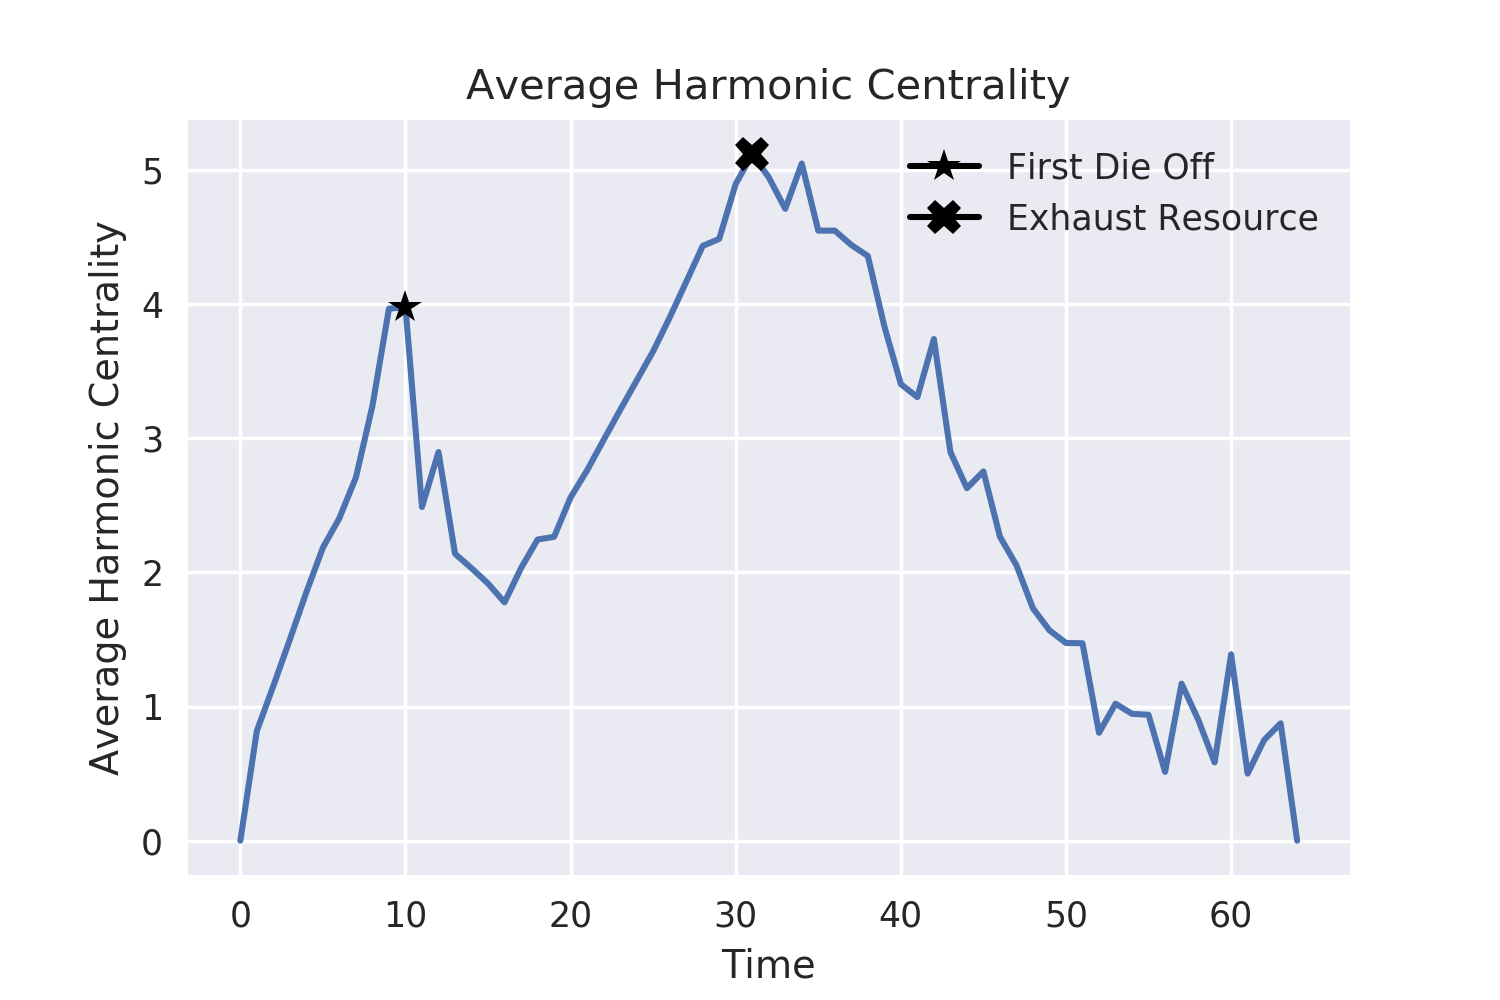
\includegraphics[scale=0.75]{harmonic_centrality.png}
		\caption{text}
		\label{harmonic}
	\end{figure}
	
	\begin{figure}[h]
		\centering
		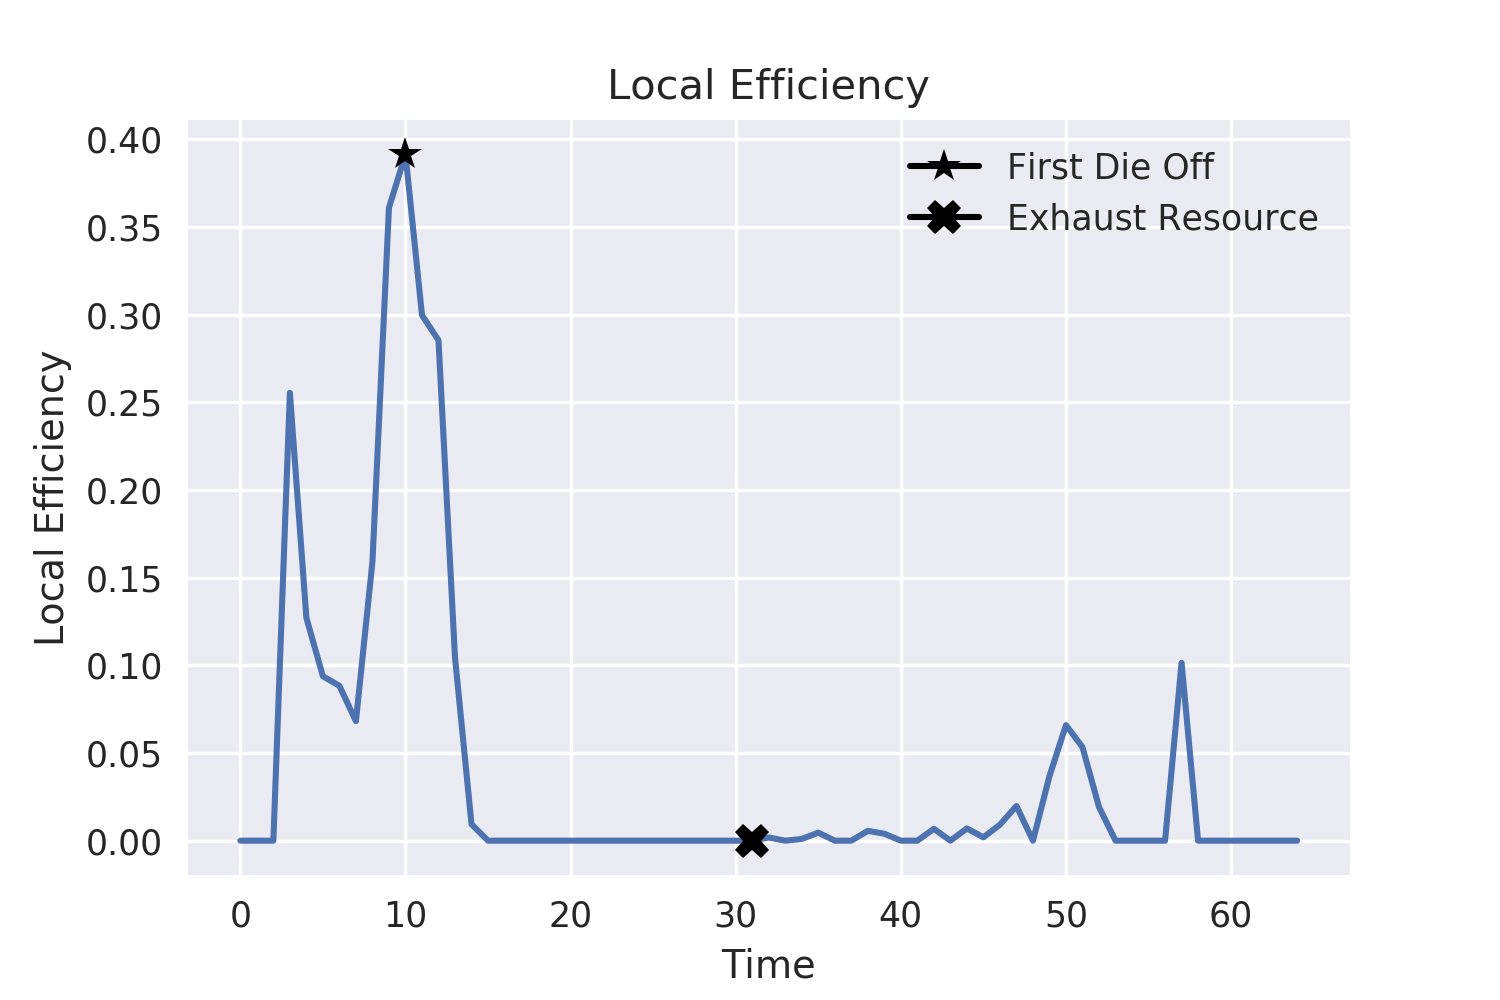
\includegraphics[scale=0.75]{local_efficiency.png}
		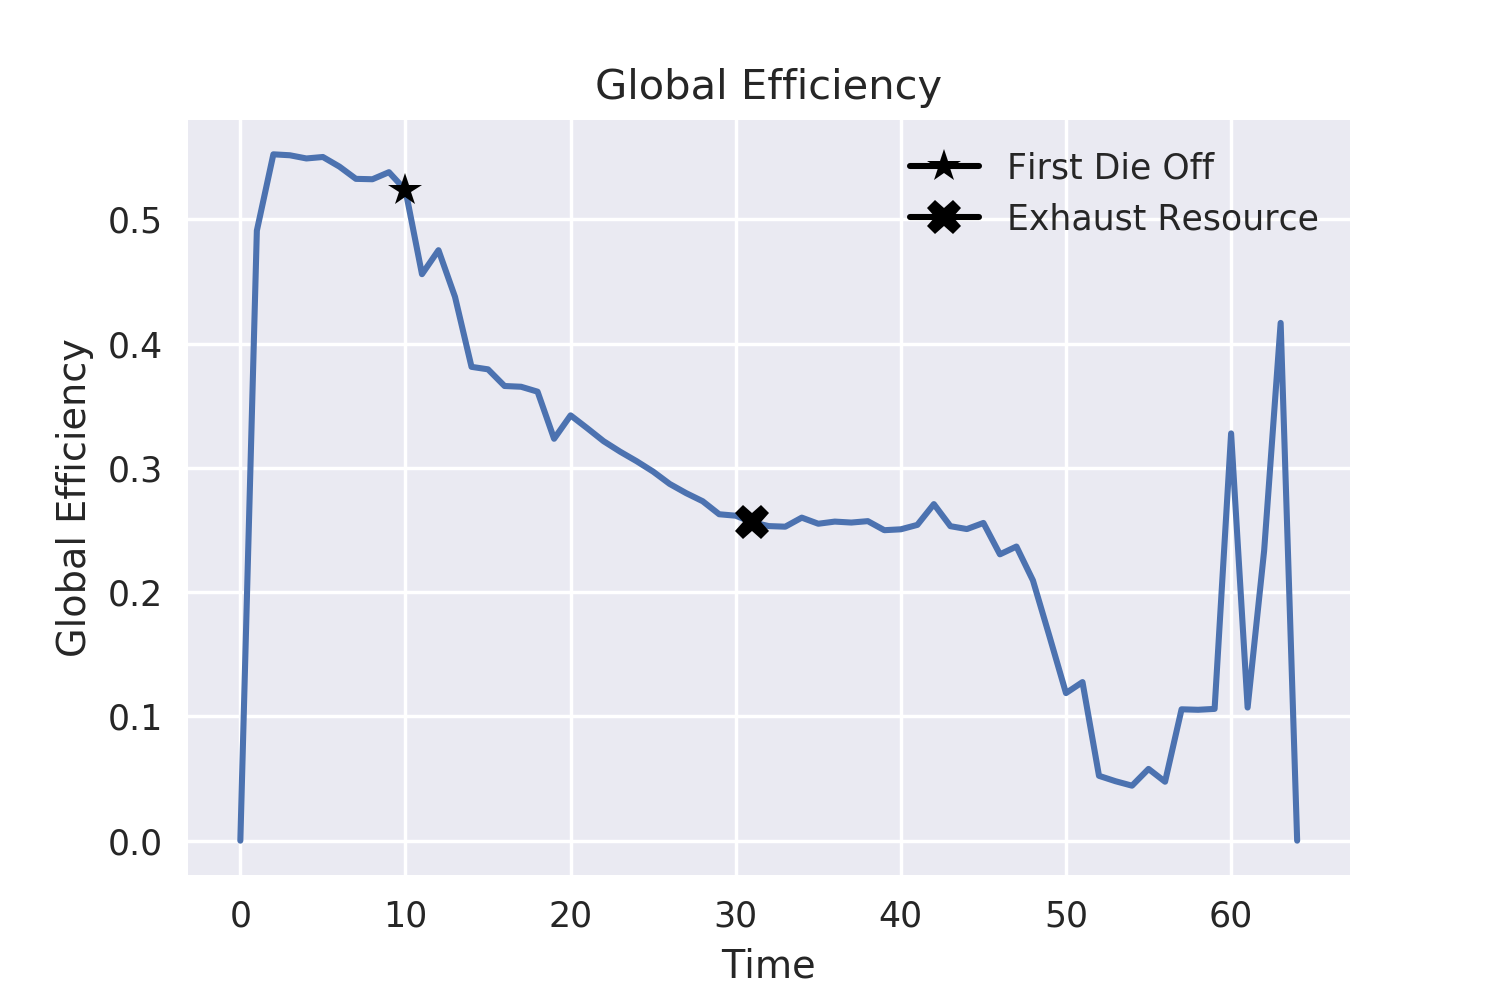
\includegraphics[scale=0.75]{global_efficiency.png}
		\text{Not sure what to say about this one}
		\label{efficiency}
	\end{figure}
	
	\subsubsection{Correlating Measures Through Time}
	While many of these measures showed similar patterns (a maxima/minima near the initial die-off, a less dramatic peak near the moment of resource exhaustion), it was not immediately apparent how these various measures related to each-other. To explore this relational space, we created trajectories of the networks through phase-space, by plotting metrics at each moment against each-other. In some cases, clear, well-defined trajectories were visible, typically when comparing the normalized entropy to some other value. For instance, the relationship between the normalized entropy and mean of the degree distribution show a highly non-trivial pattern (Figure \ref{entropy-mean}). 
	
	\begin{figure}[h]
		\centering
		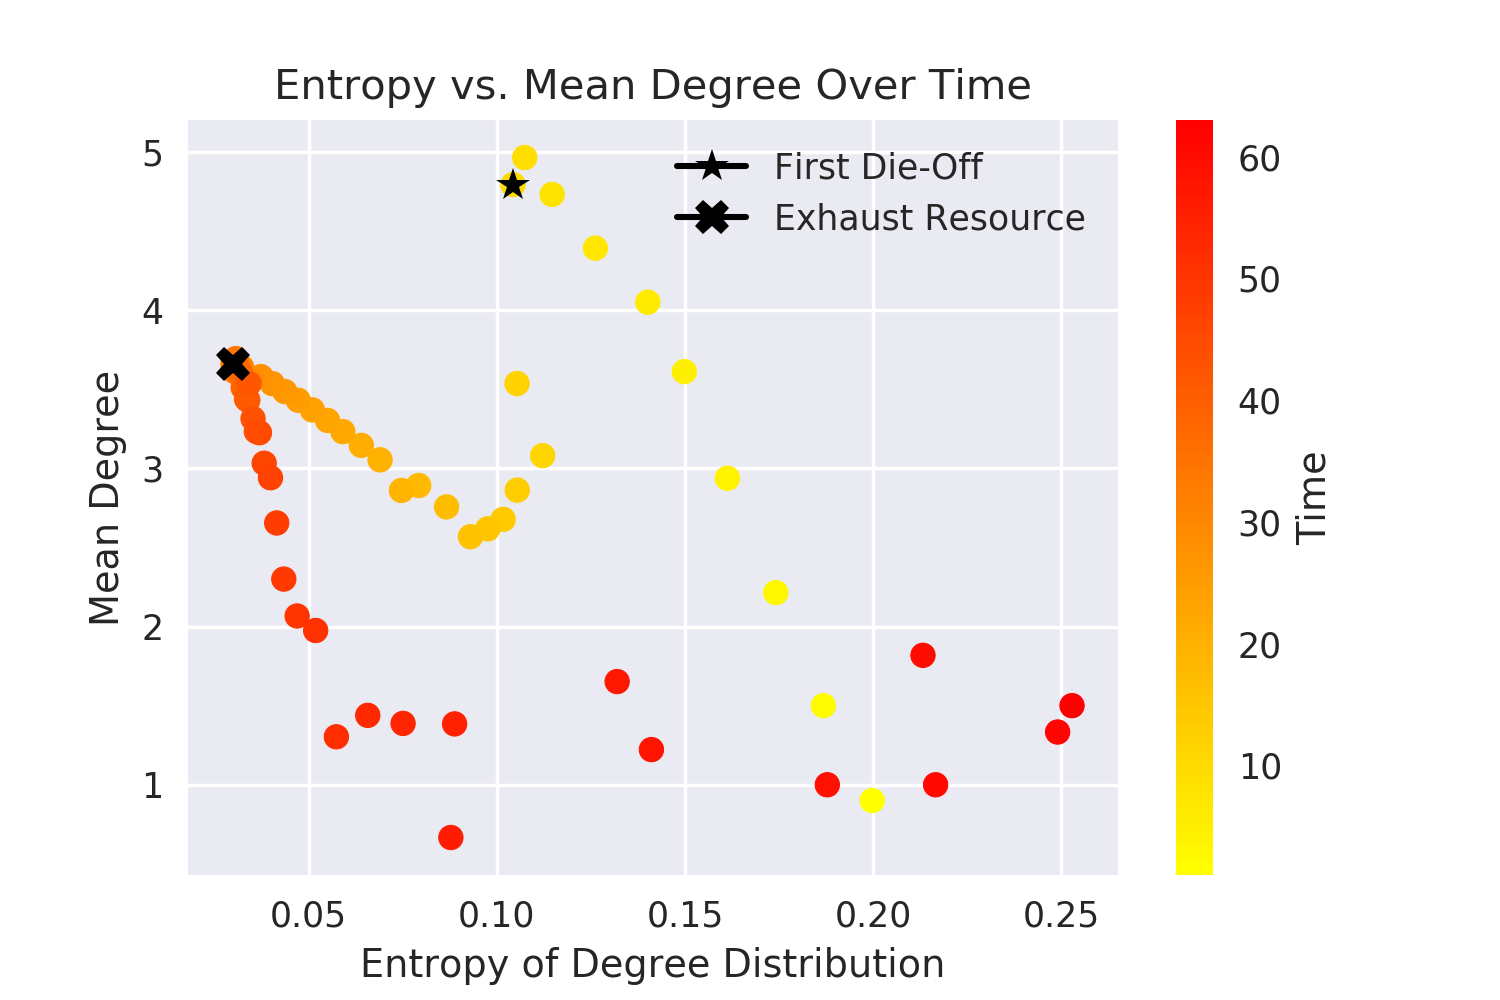
\includegraphics[scale=0.75]{ent_mean_degree.png}
		\caption{At every moment in time, the mean degree of the network, plotted against the normalized entropy of the degree distribution. The pattern begins with the most saturated yellow points, and transitions through orange to red. Note the two spikes, or sharp turns, at each of the key events, the die-off and the exhaustion of the resource nodes.}
		\label{entropy-mean}
	\end{figure}
	
	A very similar pattern was visible when plotting the variance of the degree distribution against the normalized entropy (Figure \ref{entropy-variance}). 
	
	\begin{figure}[h]
		\centering
		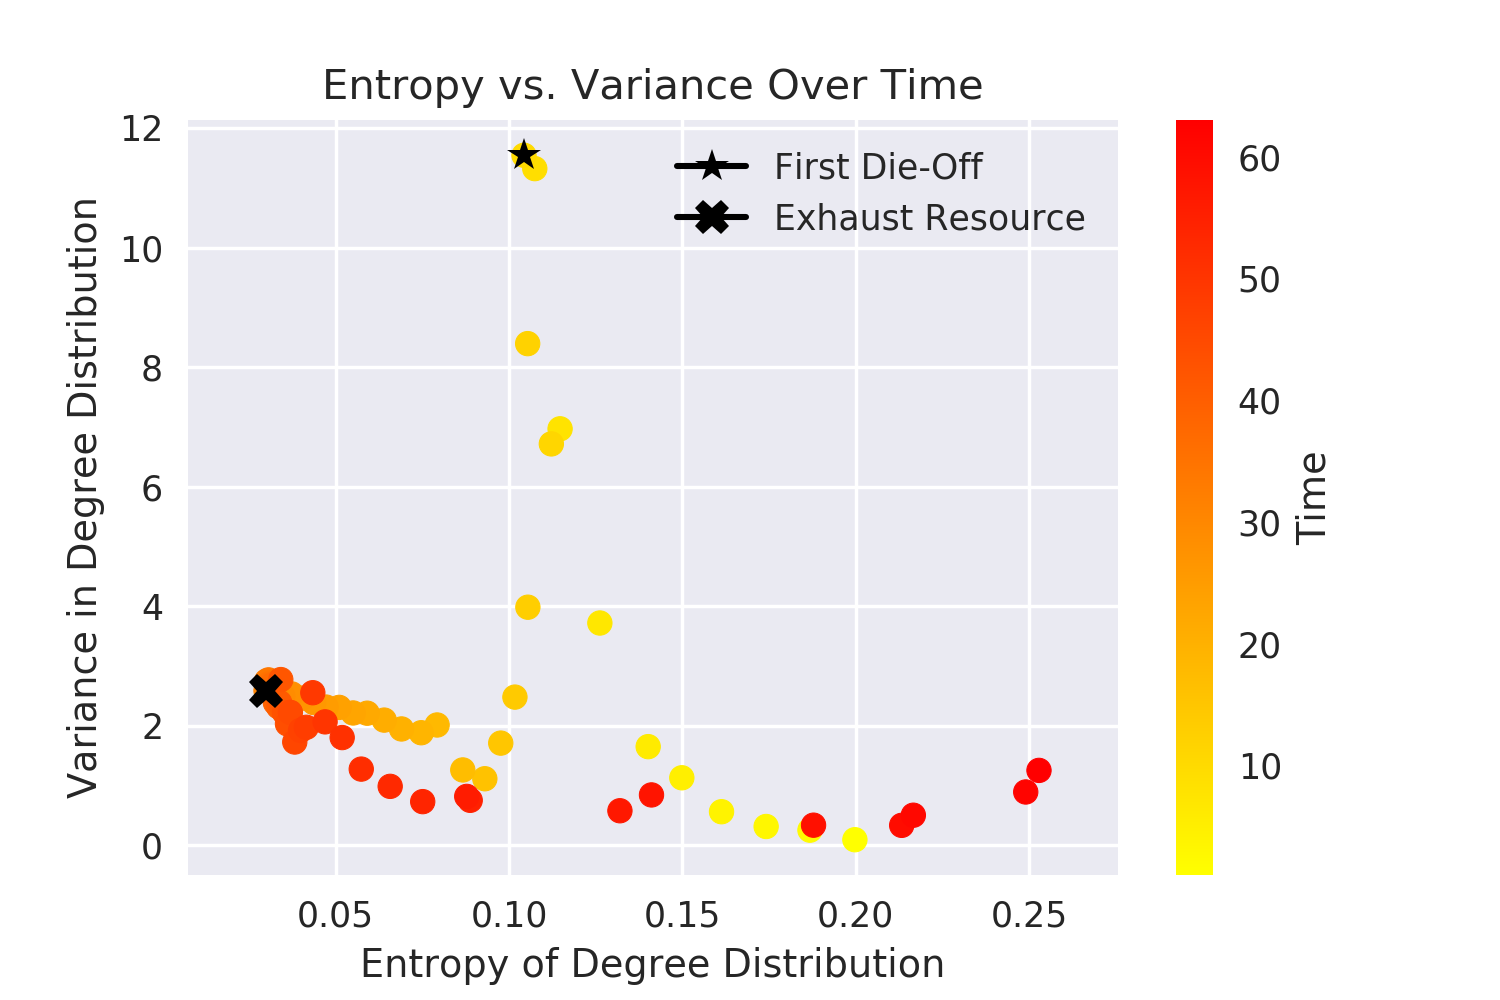
\includegraphics[scale=0.75]{ent_var_degree.png}
		\caption{The variance of the degree distribution at each moment in time plotted as a function of the entropy of the degree distribution. Here, two competing dynamics are visible: variance spikes dramatically near the initial die-off, while entropy is less affected and continues to drift downwards, until the resource node is exhausted, at which point, entropy begins to climb again, while variance falls.}
		\label{entropy-variance}
	\end{figure}
	
	While entropy, variance, and mean degree are all direct functions of the degree distribution, and consequently might be expected to be more tightly related, entropy also showed clean trajectories when compared to some graph theoretic measures, such as algebraic connectivity (Figure \ref{entropy-algconn}). The exact nature of the relationship between entropy of the degree distribution and algebraic connectivity is unclear, although algebraic connectivity has been used as a measure of system complexity in fields such as computational neuroscience \cite{bassett_adaptive_2006}. To test the relationship in a toy model, we created ensembles of Erdos-Renyi random graphs, of various sizes, and plotted entropy against algebraic connectivity, mean degree, and variance (see Figure \ref{entropy-nulls}). While in the null models similar looking trajectories could be seen, none were obvious parallels of what we saw in our evolving system, suggesting that, at least for these few measures, the observed behaviours are truly non-trivial. 
	
	\begin{figure}[h]
		\centering
		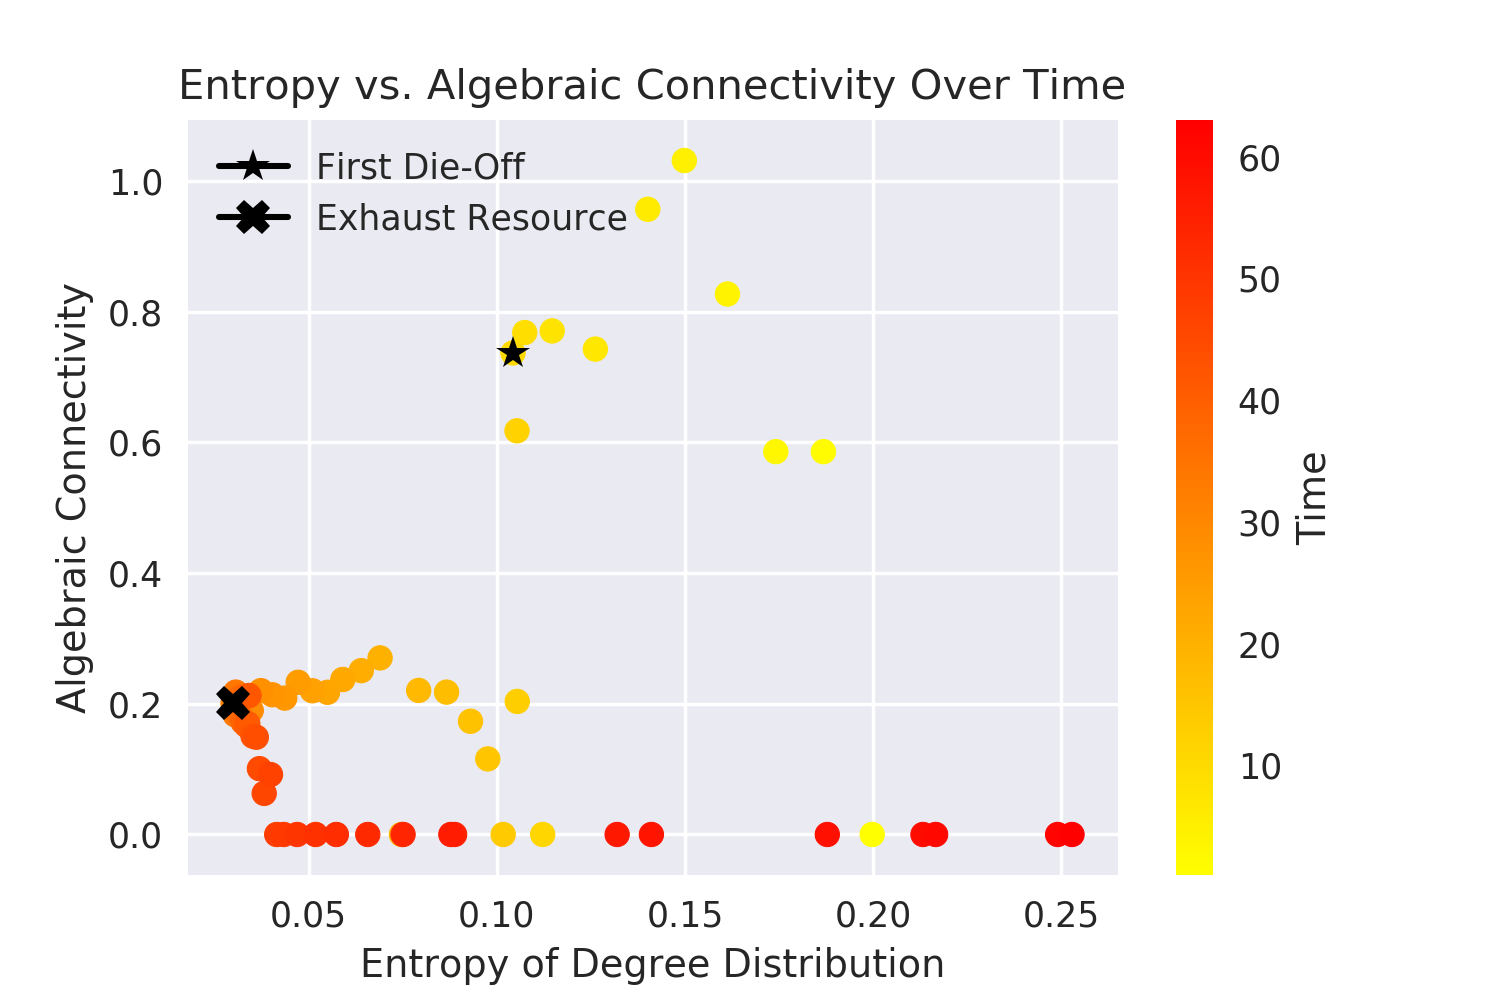
\includegraphics[scale=0.75]{ent_alg_conn.png}
		\caption{The algebraic connectivity of the network at each moment in time as a function of the entropy of the degree distribution. While the trajectory is not as clean as what is visible in Figures \ref{entropy-mean} or \ref{entropy-variance}, a clear pattern is visible. The algebraic connectivity over time is a noisier signal.}
		\label{entropy-algconn}
	\end{figure}
	
	\begin{figure}[h]
		\centering
		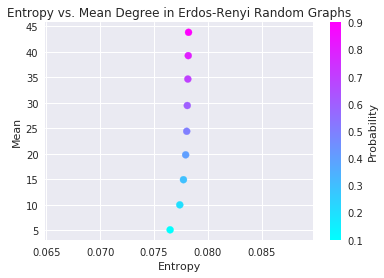
\includegraphics[scale=0.5]{null_ent_mean.png}
		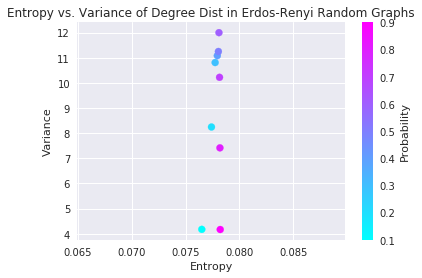
\includegraphics[scale=0.5]{null_ent_var.png}
		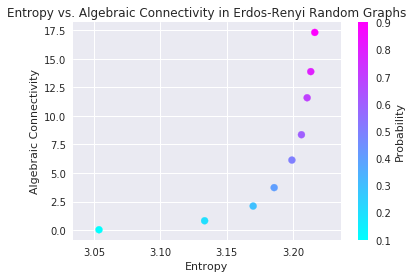
\includegraphics[scale=0.5]{null_ent_alg_conn.png}
		\caption{Simple null models plotting the relationship between entropy, mean degree, variance in degree, and algebraic connectivity of an ensemble of 25 Erdos-Renyi graphs with 50 degrees each, created with probabilities between 0.1 and 0.9}.
		\label{entropy-nulls}
	\end{figure}
	
	\subsection{Node Characteristics \& Lifetimes}
	In addition to characterizing the global behaviour of the system, we were also interested in what local structures where conducive to nodes living longer or shorter lifespans relative to their neighbours. The simplest measure to test is node creation order: are the first nodes likely to live longer, or die earlier than nodes that come into being later? For visualization, see Figure \ref{order-lifetime}. Interestingly, there seem to be two distinct 'groups' when comparing creation order to lifetime. There is a small set of nodes that are created very early (the seed population, and then a few subsequent nodes), that die very quickly. However, after the initial die-back has occurred, the network seems to find a stable structure, and subsequently, node creation order does not have an obvious effect on node lifetime (although the variance seems to climb as time goes on). This suggests that the die-back is part of a process by which the network reconfigures itself to achieve a more stable structure and dynamics. 
	
	Other measures that we explored where the average harmonic centrality of a node (which is a function of how close it is to every other node, Figure \ref{harmonic-lifetime}) and lifetime, as well as the relationship between average in- and out-degrees and lifetime (Figure \ref{degree-lifetime}), and the volume that the node consumed (Figure \ref{volume-lifetime}). In all the explored relationships, a broad similar pattern was observed: there was a small group of nodes, created early in time, that had strikingly different average scores on whatever metric we were testing, separate from the vast majority of other nodes. 
	
	As we discussed above, we interpret this as indicating that the growth phase of the network can be divided into two epochs (recall that no new nodes are created after the resource node is exhausted): the first epoch is characterized by short-lived nodes that are configured in a relatively inefficient structure, possibly due to the initialization of the system. This unstable structure collapses during the initial die-off, and is subsequently replaced by a much more stable structure, which grows until the resource node is exhausted. Within this regime, the average behaviour of the node does not show significant correlation with life-time. 
	
	\begin{figure}[h]
		\centering
		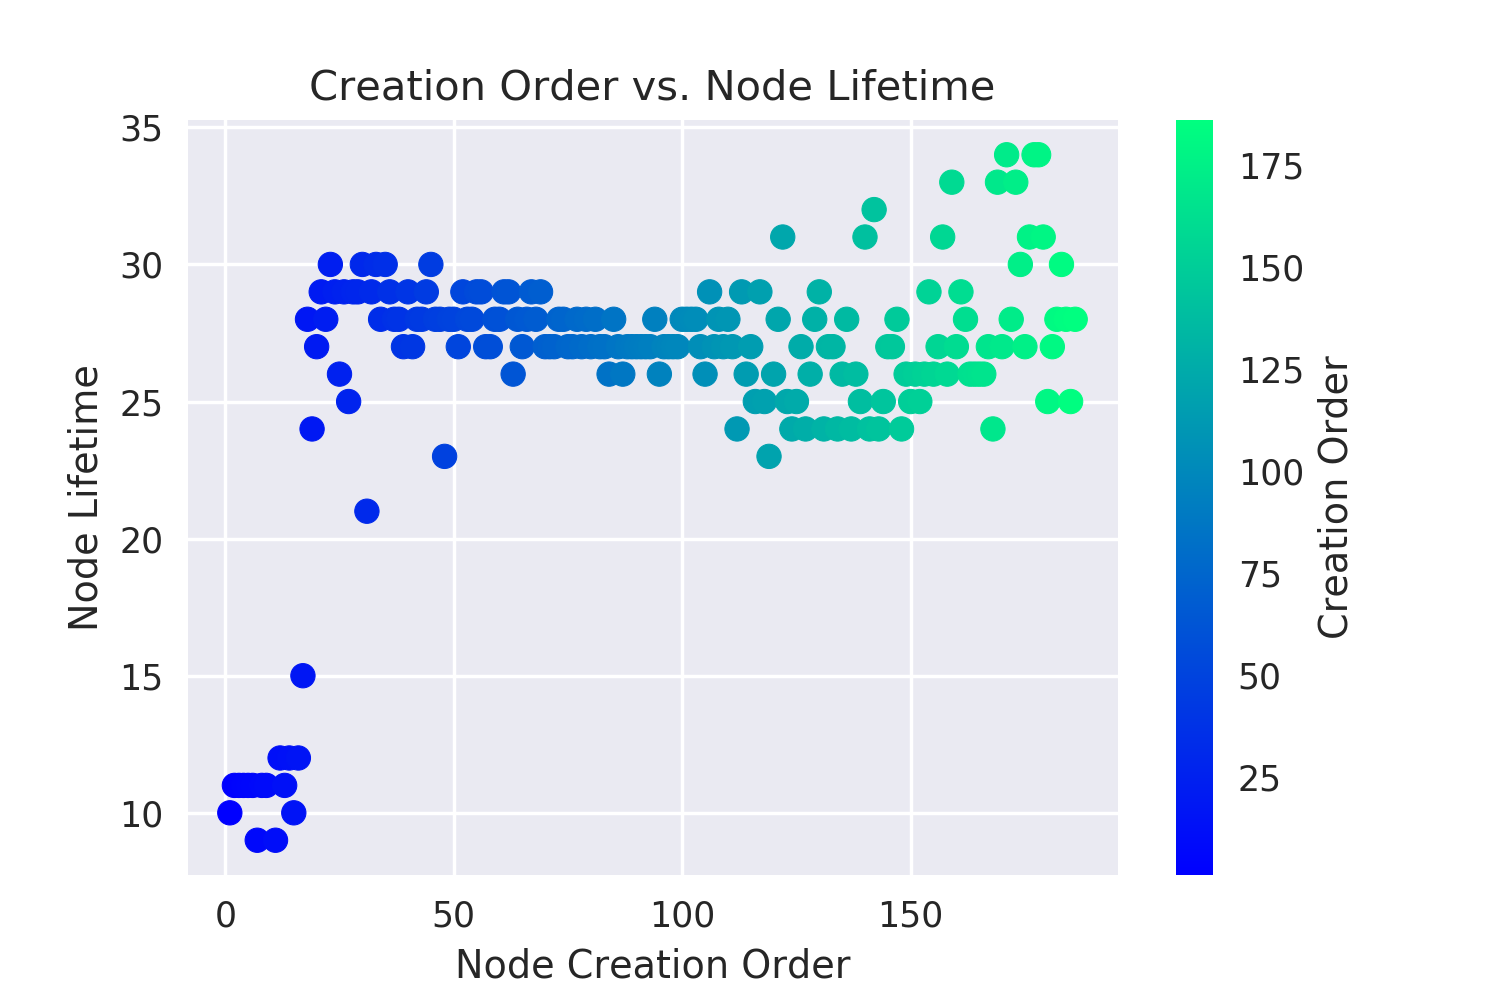
\includegraphics[scale=0.75]{creation_order_lifetimes.png}
		\caption{The lifetime of a node (how many timesteps it persisted for), plotted as a function of the order of it's creation. Node the small cluster of very early nodes with short lifetimes that are distinct from the larger set.}
		\label{order-lifetime}
	\end{figure}
	
	\begin{figure}[h]
		\centering
		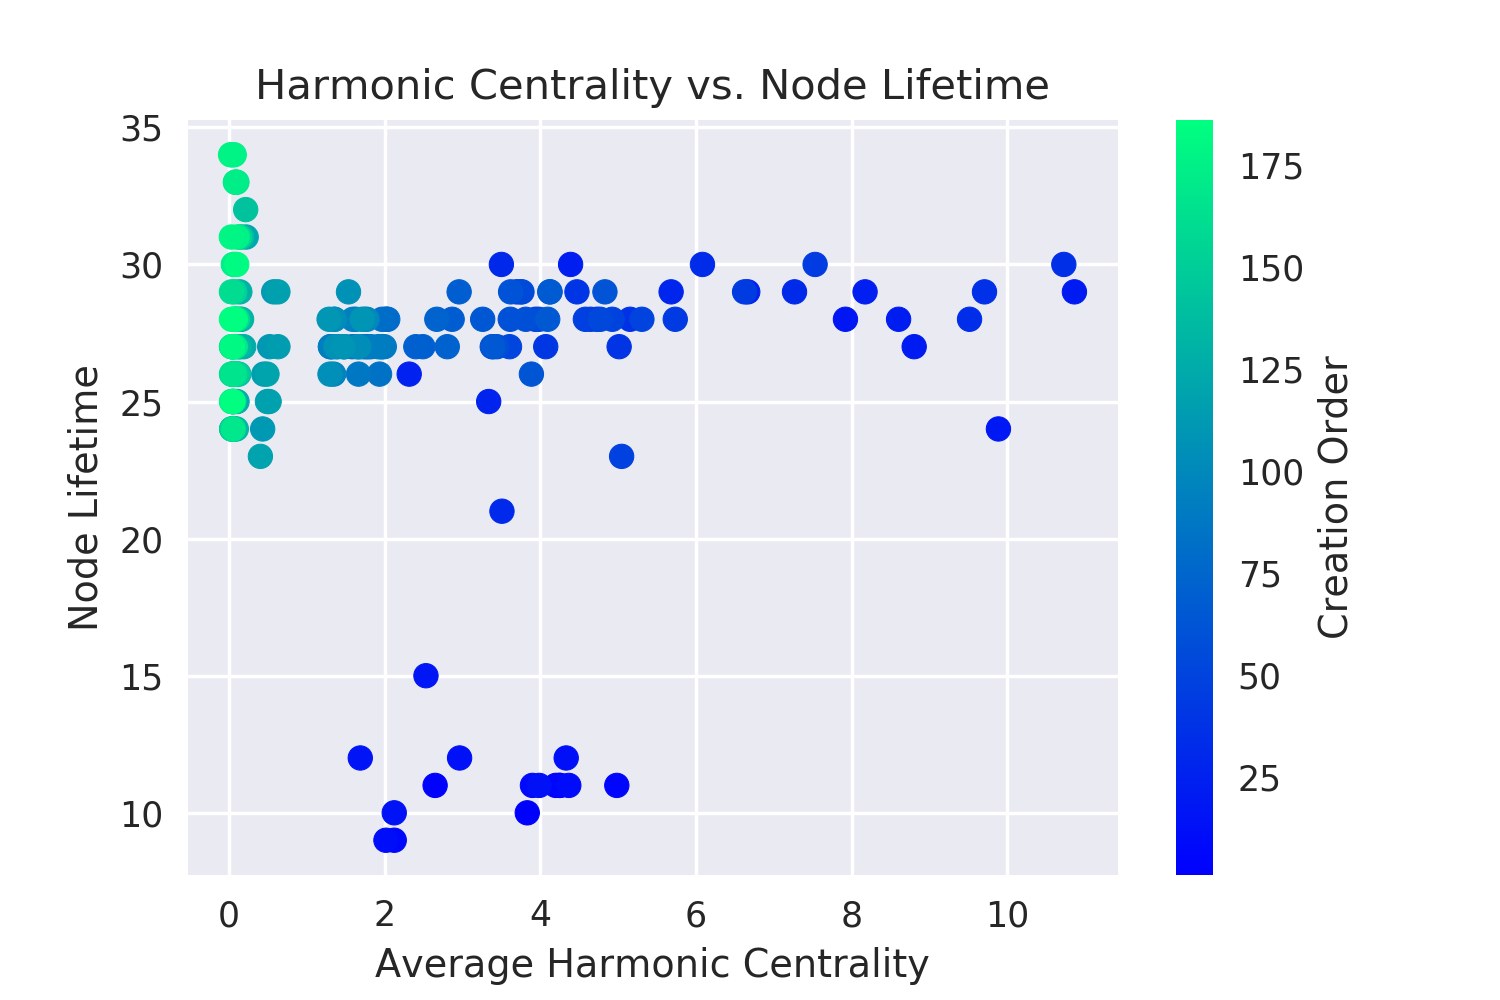
\includegraphics[scale=0.75]{harmonic_lifetimes.png}
		\caption{The average harmonic centrality of every node, plotted against the lifetime of that node, and colored based on the node creation order. As with other plots of this type, notice a small group of early nodes that don't live very long and have low harmonic centrality. There are the nodes that come into being before the initial die-off. After the die-off, an trajectory emerges, where all subsequently created nodes have roughly similar lifetimes, however, nodes created later have almost uniformly decreases average harmonic centralities. This may be reflective of the entropy described by Figure \ref{entropy}, where as time goes on, the network becomes more 'lattice-like', which less obviously central nodes.}
		\label{harmonic-lifetime}
	\end{figure}
	
	\begin{figure}[h]
		\centering
		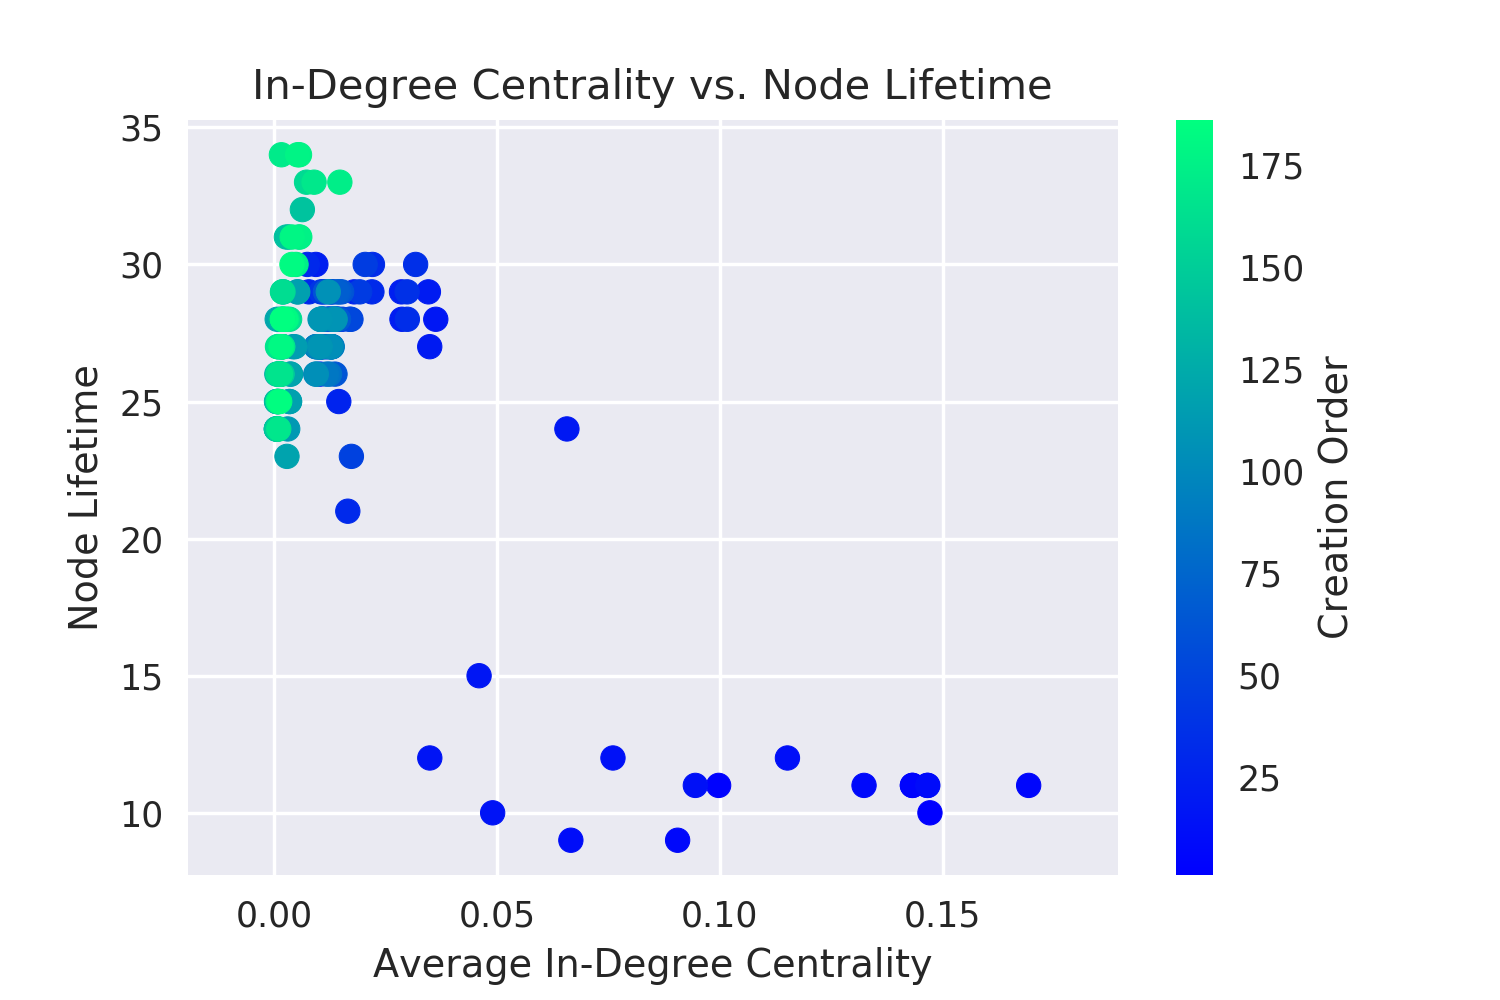
\includegraphics[scale=0.75]{in_degree_lifetimes.png}
		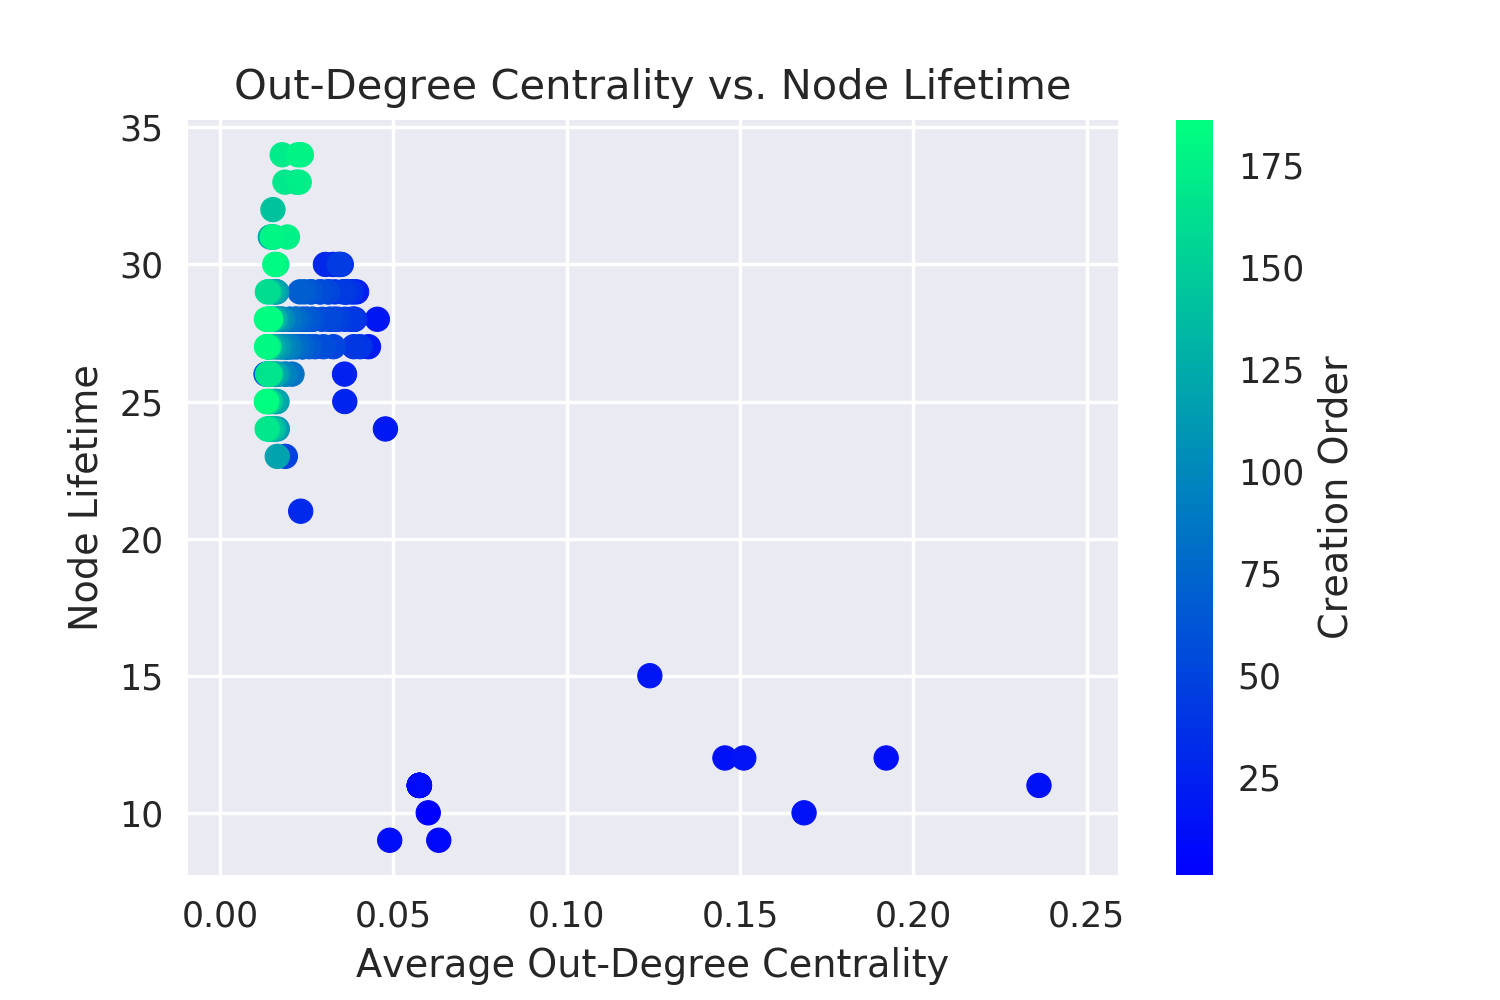
\includegraphics[scale=0.75]{out_degree_lifetimes.png}
		\caption{Here the average in- and out-degrees are plotted as a function of the node lifetime, and colored by creation order. As with other plots of this type, there is a subset of nodes created early in the history of the system that die quickly, but have high degree centralities. After the initial die-off, subsequently created nodes don't show a strong relationship between degree centrality and lifetime, although there seems to be a strong trend that nodes created later have lower in- and out-degree centralities. This is consistent with he overall homogenization described in Figures \ref{entropy} and \ref{harmonic-lifetime}.} 
		\label{degree-lifetime}
	\end{figure}
	
	\begin{figure}[h]
		\centering
		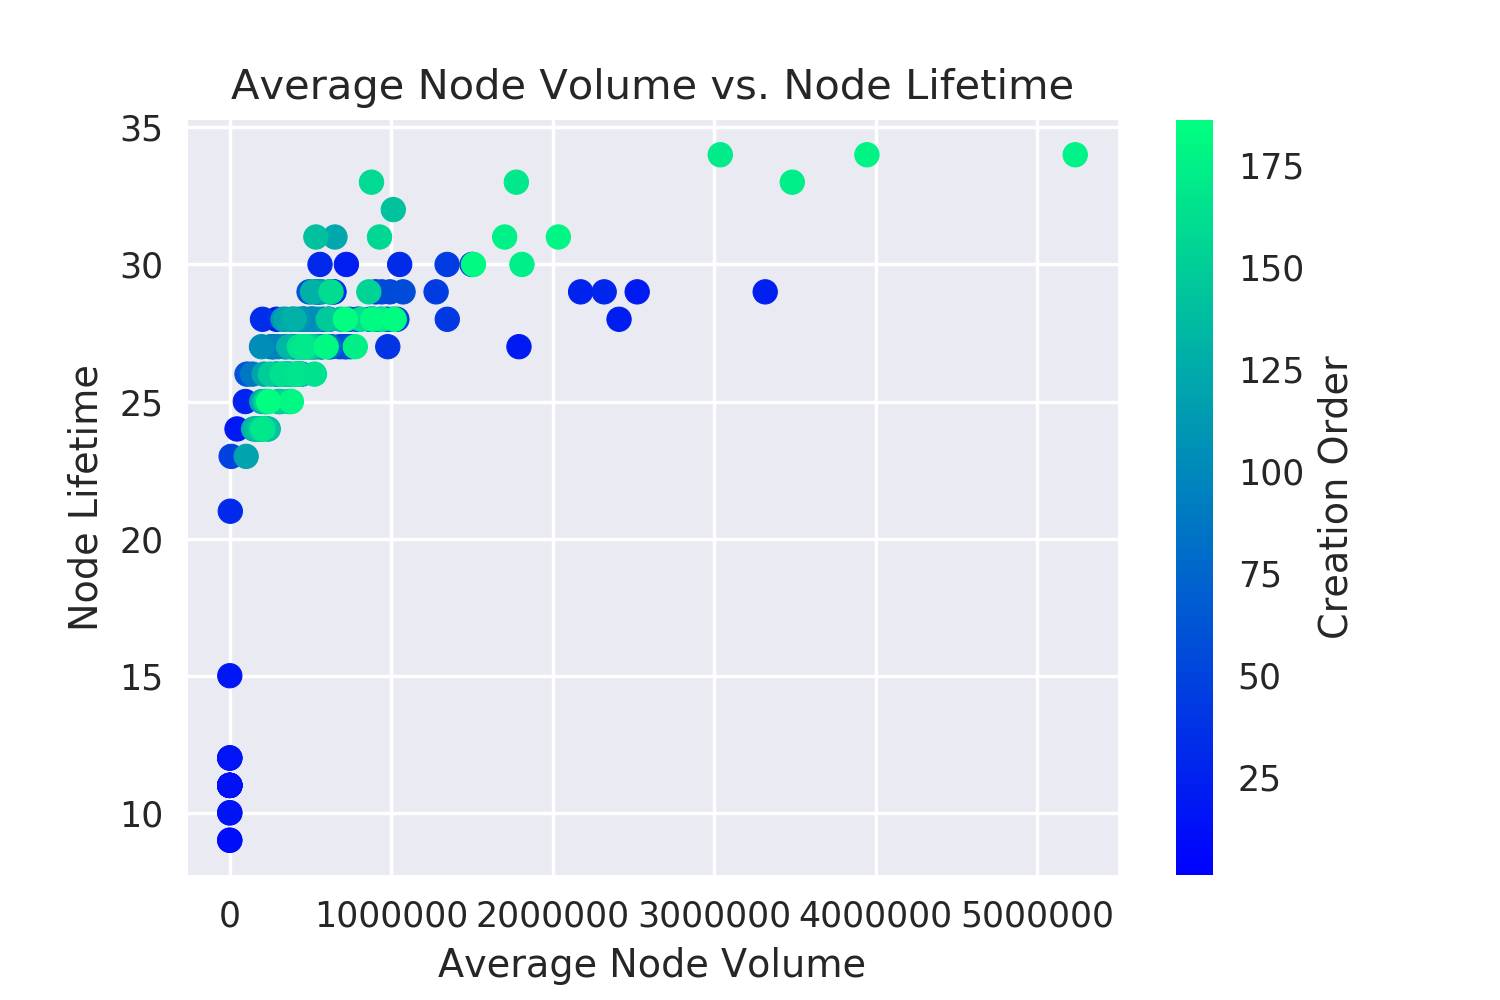
\includegraphics[scale=0.75]{volume_lifetimes.png}
		\caption{Here, the average volume of a node over the course of it's life is plotted against it's lifetime. In contrast to the various centrality plots, where after the die-off there was not a consistent relationship between metric and lifetime, here there seems to be a global, logarithmic relationship between node volume and lifetime (although the break between pre-die-off nodes and post-die-off nodes is still evident), although creation order is less tightly related to either lifetime or volume here.} 
		\label{volume-lifetime}
	\end{figure}
	
	
	\subsection{A Note on Null Models}
	Ideally, this kind of analysis would include some kind of null model, to ensure that the structures and behaviours we've observed are driven by the dissipative niche model itself and are not simply a general case of random nodes attaching themselves to the network in random orders. We struggled, however, to come up with a plausible null model that would fully capture our alternative hypothesis. The first null model we explored was, for each graph, creating an ensemble of Erdos-Renyi graphs,where the number of nodes is the same as the size of the 'real' network, and the connection probability is the edge density of the same. However, that does not capture the degree distribution, which we could not assume was binomial, or Poissonian in character. We then tried an ensemble of configuration models, running the same structural analysis. The primary problem with this model is that each moment in time is dependent on the structure of the graph at the moment before, so the connectivity and degree distributions seen in the null model are still a function of the dissipative process playing out at all previous time-steps (the ER null model shares the problem). 
	
	In future work on this project, we would want to create some kind of model that brings nodes into being randomly, attaches them to the graph randomly, and sever edges randomly, however, constructing such a model on top of our dissipative niche model proved beyond the scope of what we could accomplish here. 
	
	
	\section{Conclusions}
	
	The lifetime of the network seems to be separable into approximately three distinct phases, characterized by distinct distributions of network properties and trajectories. 
	\begin{enumerate}
		\item \textit{Initial Emergence}:
		\item \textit{Stable Growth}: The phase begins following the end of the initial die-off. In this phase, the network size begins to grow exponentially
		\item \textit{Collapse}:
	\end{enumerate}
	
	\bibliographystyle{unsrt}
	\bibliography{Dissipative_Structures.bib}
	
	\section{Appendix 1: Code}
	\lstinputlisting[language=Python]{"publishedcode.py"}
\end{document}